\documentclass{beamer}
\usepackage[utf8]{inputenc}
\usepackage[T1]{fontenc}
\usepackage{mathtools}
\usepackage{tikz}
\usepackage{amsmath}
\usepackage{braket}

\usetikzlibrary{calc,patterns,angles,quotes,quantikz}
\usepackage[backend=bibtex,
defernumbers=true,
style=verbose,
% citestyle=ieee
]{biblatex}
\addbibresource{ref.bib}
\usepackage{hyperref}

\DeclarePairedDelimiter{\ceil}{\lceil}{\rceil}

\title{Grover's Search }
\author{Selman \"Ozleyen}
\institute{Technische Universit\"at M\"unchen\\
School of Computation, Information and Technology\\}
\date{December 2022}

\addtobeamertemplate{navigation symbols}{}{%
    \usebeamerfont{footline}%
    \usebeamercolor[fg]{footline}%
    \hspace{1em}%
    \insertframenumber/\inserttotalframenumber
}

\begin{document}

\frame{\titlepage}



%%%%%%
\begin{frame}
  \frametitle{Problem Definition}
  We would like to find a specific entry from an unsorted
  database consisting of N entries. We can model this like the following:
  \begin{enumerate}
    \item Let the index of the desired element be $w$.
    % w as in winner index
    \item Let our database be a function 
    $f:[N-1]\rightarrow\{0,1\}$ s.t. $f(w)=1$ and $f(x)=0$ for all other elements.
    \item We have $f$ but we don't have $w$, so we want to find it.
  \end{enumerate}
\end{frame}
%%%%%%

% Ask audience:
% how many iterations would this require on average on a classical computer?



%%%%%%
\begin{frame}
  \frametitle{Grover's Oracle}
  We access $f$ with an \textit{oracle}. It can be written
  as a unitary operator $U_w$ defined as below,
  $$
  U_w|x\rangle = \bigg\{
    \begin{aligned}
    \phantom{-}|x\rangle \quad \text{if} \; x \neq w \\
    -|x\rangle \quad \text{if} \; x = w \\
    \end{aligned}
    $$
  Note that $|x\rangle = |x_{n-1}...\rangle|x_1\rangle |x_0\rangle$ where $n=\ceil{\log N}$.
\end{frame}
%%%%%%

%%%%%%
\begin{frame}
  \frametitle{Grover's Oracle: Example}
  \textbf{Example:}
  Consider the case when we have 8 entries and the winner index is 2. Our oracle looks like
  $$
  U_w = 
\begin{bmatrix}
1 & 0 & 0 & 0 & 0 & 0 & 0 & 0 \\
0 & 1 & 0 & 0 & 0 & 0 & 0 & 0 \\
0 & 0 & -1 & 0 & 0 & 0 & 0 & 0 \\
0 & 0 & 0 & 1 & 0 & 0 & 0 & 0 \\
0 & 0 & 0 & 0 & 1 & 0 & 0 & 0 \\
0 & 0 & 0 & 0 & 0 & 1 & 0 & 0 \\
0 & 0 & 0 & 0 & 0 & 0 & 1 & 0 \\
0 & 0 & 0 & 0 & 0 & 0 & 0 & 1 \\
\end{bmatrix}
  $$
% remind: counting starts from zero
\end{frame}
%%%%%%




%%%%%%
\begin{frame}
  \frametitle{Quantum Oracles}
  In general, such quantum oracles for search algorithms are usually written as the following.
  \begin{enumerate}
    \item Let $f(x)$ be a classical function s.t. $f(x)=1$ if $x$ is what we search for, else $f(x)=0$.
    \item There can be more than one $x$ s.t. $f(x)=1$ in general.
    \item Usually, the effect is written as $U_f|x\rangle = (-1)^{f(x)}|x\rangle$.
    \item We focus on the case when there is only one solution.
    \item But the algorithm also works for multiple solutions!  
    %  as in Grover's work.
  \end{enumerate}
  In short, Quantum Oracles flip the phase of the solution state.
% CITE BOOK
\end{frame}
%%%%%%

%%%%%%
\begin{frame}
  \frametitle{Grover's Oracle in Practice}
  How to implement an oracle without knowing the solution?
  \begin{enumerate}
    \item Create a classical (possibly irreversible) circuit that recognizes the solution.
    \item Construct a reversible classical circuit from it.
    \item Use \textit{phase kickback} and \textit{uncomputation} to turn this circuit into an oracle\footcite[]{book}.
  \end{enumerate}
  We won't cover the details of \textit{phase kickback} and \textit{uncomputation} concepts. 
  % cite notebook

% Phase kickback: Applying a controlled gate to qubits in a certain state can actually change the phase of the control qubit
% Uncomputation: Do parts of the computation in reverse to get the working qubits back to a |0> state
\end{frame}
%%%%%%

%%%%%%
\begin{frame}
  \frametitle{Grover's Oracle in Practice: Wrap Up}

But in general we should know that 
\begin{enumerate}[.]
  \item It is easy to convert a problem into an oracle form.
  \item Because we don't need to find the solution, verifying it is usually enough \footcite[]{Qiskit}.
  \item For example, we can create a circuit to verify a Sudoku solution.
  \item Which is much easier than finding a Sudoku solution.
\end{enumerate}
% cite notebook
\end{frame}
%%%%%%

%%%%%%
\begin{frame}
  \frametitle{Algorithm Outline}
  Grover's algorithm can be summarized as two stages.
  \begin{enumerate}
    \item Create a quantum oracle.
    \item Apply \textit{amplitude amplification}
  \end{enumerate}
  In the following, we will cover amplitude amplification.
\end{frame}
%%%%%%


%%%%%%
\begin{frame}
  \frametitle{Amplitude Amplification: Operators \& Notation}
  Let $\boldsymbol{|s\rangle}=\frac{1}{\sqrt{N}} \sum_{x = 0}^{N -1} | \boldsymbol{x} \rangle$ 
  and  $\boldsymbol{|s'\rangle}=\frac{1}{\sqrt{N-1}} \sum_{x \neq w} | \boldsymbol{x} \rangle$.
  We define the following operators:

  \begin{enumerate}[(i)]
    \item  $U_s=2|\boldsymbol s\rangle\langle \boldsymbol s| - I$
    \item  $U_w=I-2|\boldsymbol w\rangle\langle \boldsymbol w|$ 
  \end{enumerate}
  Notice that $U_w$ is still the oracle, just written differently.
\end{frame}
%%%%%%


%%%%%%
\begin{frame}
  \frametitle{Amplitude Amplification: Geometric View}
  % we know that these are orthogonal.
  \hspace*{\fill}  Recall that $\boldsymbol{|s\rangle}=\frac{1}{\sqrt{N}} \sum_{x = 0}^{N -1} | \boldsymbol{x} \rangle$ \\
  \hspace*{\fill}  and $\boldsymbol{|s'\rangle}=\frac{1}{\sqrt{N-1}} \sum_{x \neq w} | \boldsymbol{x} \rangle$.
  


  \begin{tikzpicture}
    \coordinate (origin) at (0,0);
    \coordinate (w) at (0,5);
    \coordinate (sprime) at (5,0);
    \coordinate (s) at (4,2);
    \coordinate (Uws) at (4,-2);

    \draw[line width=1pt,black,-stealth](origin)--(w) node[anchor=south west]{$\boldsymbol{|w\rangle}$};
    \draw[line width=1pt,black,-stealth](origin)--(sprime) node[anchor=north east]{$\boldsymbol{|s'\rangle}$};
  \end{tikzpicture}
  % \hspace*{\fill}  Notice that $\boldsymbol{|s'\rangle}$ is perpendicular to $\boldsymbol{|w\rangle}$.

\end{frame}
%%%%%%

%%%%%%
\begin{frame}
  \frametitle{Amplitude Amplification: Geometric View}
  \hspace*{\fill} We know that $\boldsymbol{|s\rangle}$ lies between $\boldsymbol{|w\rangle}$ and $\boldsymbol{|s'\rangle}$
  
  \begin{tikzpicture}
    \coordinate (origin) at (0,0);
    \coordinate (w) at (0,5);
    \coordinate (sprime) at (5,0);
    \coordinate (s) at (4,2);
    \coordinate (Uws) at (4,-2);
    \draw[line width=1pt,black,-stealth](origin)--(w) node[anchor=south west]{$\boldsymbol{|w\rangle}$};
    \draw[line width=1pt,black,-stealth](origin)--(sprime) node[anchor=north east]{$\boldsymbol{|s'\rangle}$};
    \draw[line width=1pt,black,-stealth](origin)--(s) node[anchor=south west]{$\boldsymbol{|s\rangle}$};
  \end{tikzpicture}
\end{frame}
%%%%%%


%%%%%%
\begin{frame}
  % s lies between them.
  % 
  \frametitle{Amplitude Amplification: Geometric View}
  \hspace*{\fill} Let's denote the angle between  $\boldsymbol{|s\rangle}$ and $\boldsymbol{|s'\rangle}$ as $\theta/2$

  \begin{tikzpicture}
    \coordinate (origin) at (0,0);
    \coordinate (w) at (0,5);
    \coordinate (sprime) at (5,0);
    \coordinate (s) at (4,2);
    \coordinate (Uws) at (4,-2);
   
    \draw (sprime) coordinate (A) -- (origin) coordinate (B)
         -- (s) coordinate (C)
           pic ["$\theta/2$", draw,black,thick,angle radius=2cm] {angle = A--B--C};

    \draw[line width=1pt,black,-stealth](origin)--(w) node[anchor=south west]{$\boldsymbol{|w\rangle}$};
    \draw[line width=1pt,black,-stealth](origin)--(s) node[anchor=south west]{$\boldsymbol{|s\rangle}$};
    \draw[line width=1pt,black,-stealth](origin)--(sprime) node[anchor=south west]{$\boldsymbol{|s'\rangle}$};
  \end{tikzpicture}
\end{frame}
%%%%%%


%%%%%%
\begin{frame}
  \frametitle{Amplitude Amplification: Geometric View}
  \hspace*{\fill} We apply $U_w$ to $\boldsymbol{|s\rangle}$ 
  because it acts as a 
  \\ \hspace*{\fill}
  reflection across $\boldsymbol{|s'\rangle}$.
  % Notice how they are always in the space of sprime and w


  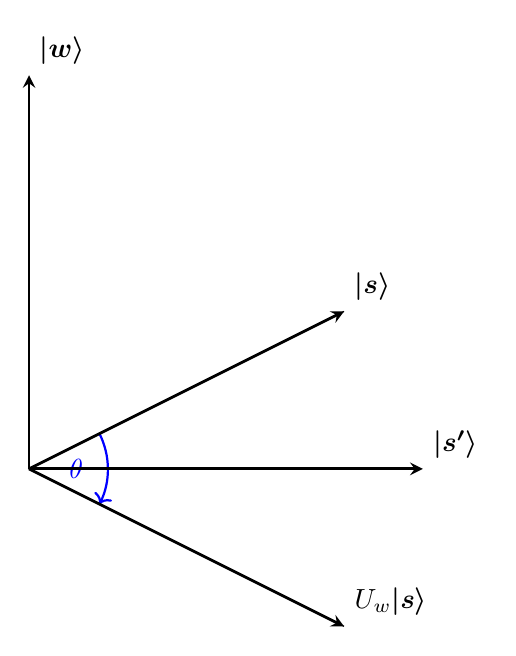
\begin{tikzpicture}
    \coordinate (origin) at (0,0);
    \coordinate (w) at (0,5);
    \coordinate (sprime) at (5,0);
    \coordinate (s) at (4,2);
    \coordinate (Uws) at (4,-2);
   
    \draw (Uws) coordinate (A) -- (origin) coordinate (B)
    -- (s) coordinate (C)
      pic ["$\theta$", draw,<-,blue,thick,angle radius=1cm] {angle = A--B--C};

    \draw[line width=1pt,black,-stealth](origin)--(w) node[anchor=south west]{$\boldsymbol{|w\rangle}$};
    \draw[line width=1pt,black,-stealth](origin)--(s) node[anchor=south west]{$\boldsymbol{|s\rangle}$};
    \draw[line width=1pt,black,-stealth](origin)--(sprime) node[anchor=south west]{$\boldsymbol{|s'\rangle}$};
    \draw[line width=1pt,black,-stealth](origin)--(Uws) node[anchor=south west]{$U_w\boldsymbol{|s\rangle}$};
  \end{tikzpicture}
\end{frame}
%%%%%%


%%%%%%
\begin{frame}
  \frametitle{Amplitude Amplification: Geometric View}
  \hspace*{\fill} Then we apply $U_s$ to $U_w\boldsymbol{|s\rangle}$
  which acts as a 
  \\ \hspace*{\fill}
  reflection across $\boldsymbol{|s\rangle}$.


  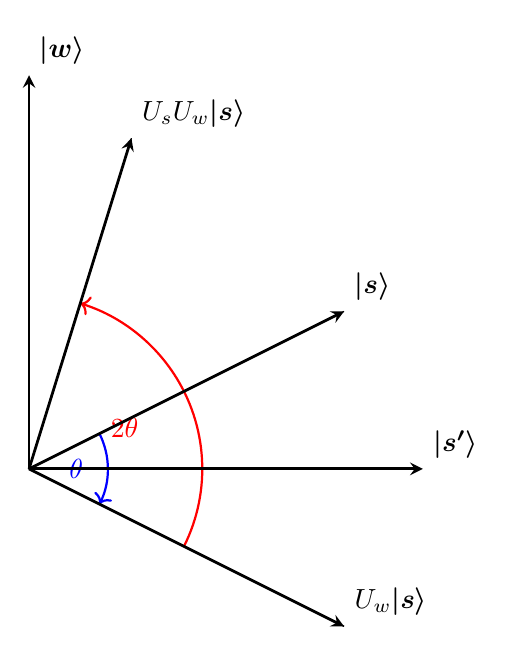
\begin{tikzpicture}
    \coordinate (origin) at (0,0);
    \coordinate (w) at (0,5);
    \coordinate (sprime) at (5,0);
    \coordinate (s) at (4,2);
    \coordinate (Uws) at (4,-2);
    \coordinate (UsUws) at (1.3,4.2);
   
    \draw (Uws) coordinate (A) -- (origin) coordinate (B)
    -- (UsUws) coordinate (C)
      pic ["$2\theta$", draw,->,red,thick,angle radius=2.2cm] {angle = A--B--C};
    \draw (s) coordinate (A) -- (origin) coordinate (B)
    -- (Uws) coordinate (C)
      pic ["$\theta$", draw,<-,blue,thick,angle radius=1cm] {angle = C--B--A};

    \draw[line width=1pt,black,-stealth](origin)--(w) node[anchor=south west]{$\boldsymbol{|w\rangle}$};
    \draw[line width=1pt,black,-stealth](origin)--(s) node[anchor=south west]{$\boldsymbol{|s\rangle}$};
    \draw[line width=1pt,black,-stealth](origin)--(sprime) node[anchor=south west]{$\boldsymbol{|s'\rangle}$};
    \draw[line width=1pt,black,-stealth](origin)--(Uws) node[anchor=south west]{$U_w\boldsymbol{|s\rangle}$};
    \draw[line width=1pt,black,-stealth](origin)--(UsUws) node[anchor=south west]{$U_sU_w\boldsymbol{|s\rangle}$};
  \end{tikzpicture}
\end{frame}
%%%%%%

%%%%%%
\begin{frame}
  \frametitle{Amplitude Amplification: Geometric View}
  \hspace*{\fill} The $\boldsymbol{\ket{s}}$ had a magnitude of $\sin{(\theta/2)}$ on $\boldsymbol{\ket{w}}$. The result \\ 
  \hspace*{\fill} $U_sU_w\boldsymbol{\ket{s}}$ has magnitude of $\sin{(3\theta/2)}$ on $\boldsymbol{\ket{w}}$


  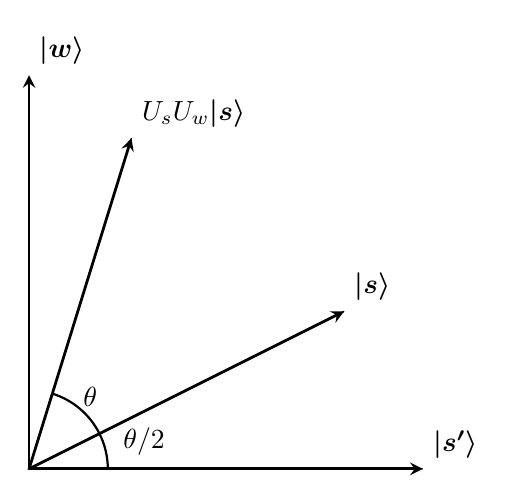
\begin{tikzpicture}
    \coordinate (origin) at (0,0);
    \coordinate (w) at (0,5);
    \coordinate (sprime) at (5,0);
    \coordinate (s) at (4,2);
    \coordinate (Uws) at (4,-2);
    \coordinate (UsUws) at (1.3,4.2);
   
    \draw (s) coordinate (A) -- (origin) coordinate (B)
    -- (UsUws) coordinate (C)
      pic ["$\theta$", draw,black,thick,angle radius=1cm, angle eccentricity=1.2] {angle = A--B--C};
    \draw (s) coordinate (A) -- (origin) coordinate (B)
    -- (sprime) coordinate (C)
      pic ["$\theta/2$", draw,black,thick,angle radius=1cm, angle eccentricity=1.5] {angle = C--B--A};
    
    \draw[line width=1pt,black,-stealth](origin)--(w) node[anchor=south west]{$\boldsymbol{|w\rangle}$};
    \draw[line width=1pt,black,-stealth](origin)--(s) node[anchor=south west]{$\boldsymbol{|s\rangle}$};
    \draw[line width=1pt,black,-stealth](origin)--(sprime) node[anchor=south west]{$\boldsymbol{|s'\rangle}$};
    \draw[line width=1pt,black,-stealth](origin)--(UsUws) node[anchor=south west]{$U_sU_w\boldsymbol{|s\rangle}$};
  \end{tikzpicture}
\end{frame}
%%%%%%

%%%%%%
\begin{frame}
  \frametitle{Amplitude Amplification: Applying Iterations}
  $U_sU_w\boldsymbol{\ket{s}}$ has magnitude of $\sin{(3\theta/2)}$ on $\boldsymbol{\ket{w}}$.
  \begin{enumerate}[-]
    \item After $r$ iterations.
    \item $(U_sU_w)^r\boldsymbol{\ket{s}}$ will have a magnitude of $\sin{\left(\theta(r+1/2)\right)}$ on $\boldsymbol{\ket{w}}$.
  \end{enumerate}
\end{frame}
%%%%%%

%%%%%%
\begin{frame}
  \frametitle{Amplitude Amplification: Finding Number of Iterations}
  Following from the previous results, we conclude:
  \begin{enumerate}[-]
    \item The probability of measuring the solution is $\sin{\left(\theta\left(r+1/2\right)\right)}^2$.
    \item By our definition of $\theta$, we know $\theta = 2 \arcsin{\frac{1}{\sqrt{N}}}$.
    \item We use this to maximize $\sin{\left(\theta\left(r+1/2\right)\right)}^2$ w.r.t $r$.
    \item This is maximized when we set $r \approx \pi\sqrt{N}/4$.
  \end{enumerate}
  So we need $O(\sqrt{N})$ iterations to measure the solution with high probability.
  One can also show that the error is $O(1/N)$\footcite[]{Grover_1997}.
\end{frame}
%%%%%%

\newcommand{\Uw}{\gate[wires=3, style={fill=red!15}]{U_w}}
\newcommand{\Us}{\gate[wires=3, style={fill=blue!15}]{U_s}}

%%%%%%
\begin{frame}
  \frametitle{Grover's Algorithm}
  To find our solution in $O(\sqrt{N})$ steps we:
  \begin{enumerate}
    \item Create a quantum oracle $U_w$
    \item Compute $(U_sU_w)^r\boldsymbol{\ket{s}}$ with appropriate amount of $r$.
    \item Measure the result.
  \end{enumerate}
  \vspace{1cm}
  \begin{center}
      \begin{quantikz}[transform canvas={scale=0.6}]
        \lstick{$\ket{0}$} & \gate{H} & \Uw & \Us & \Uw & \Us & \qw & & & \Uw & \Us & \meter{}\\
        \lstick{$\ket{0}$} & \gate{H} & & & & & \qw & \ldots & & & & \meter{}\\
        \lstick{$\ket{0}$} & \gate{H} & & & & & \qw & & & & & \meter{}
        \end{quantikz}
  \end{center}
  
  
\end{frame}
%%%%%%

%%%%%%
\begin{frame}
  \frametitle{Summary}
  We will see how this algorithm can be done in a quantum circuit. But to summarize until now:
  \begin{enumerate}[-]
    \item It is conceptually easy to create a quantum oracle from classical circuits.
    \item Quantum computers can find an entry from an unsorted database in $O(\sqrt{N})$ iterations.
    \item While classical computers need $O(N)$.
  \end{enumerate}
\end{frame}
%%%%%%


\begin{frame}
\frametitle{References}
% This prints the bibliography on the slide
\printbibliography
\end{frame}

\end{document}